\documentclass[12pt,]{article}
\usepackage[T1]{fontenc}
\usepackage{lmodern}
\usepackage{amssymb,amsmath}
\usepackage{ifxetex,ifluatex}
\usepackage{fixltx2e} % provides \textsubscript
% use upquote if available, for straight quotes in verbatim environments
\IfFileExists{upquote.sty}{\usepackage{upquote}}{}
\ifnum 0\ifxetex 1\fi\ifluatex 1\fi=0 % if pdftex
  \usepackage[utf8]{inputenc}
\else % if luatex or xelatex
  \ifxetex
    \usepackage{mathspec}
    \usepackage{xltxtra,xunicode}
  \else
    \usepackage{fontspec}
  \fi
  \defaultfontfeatures{Mapping=tex-text,Scale=MatchLowercase}
  \newcommand{\euro}{€}
\fi
% use microtype if available
\IfFileExists{microtype.sty}{\usepackage{microtype}}{}
\usepackage[margin=1in]{geometry}
\usepackage{graphicx}
% Redefine \includegraphics so that, unless explicit options are
% given, the image width will not exceed the width of the page.
% Images get their normal width if they fit onto the page, but
% are scaled down if they would overflow the margins.
\makeatletter
\def\ScaleIfNeeded{%
  \ifdim\Gin@nat@width>\linewidth
    \linewidth
  \else
    \Gin@nat@width
  \fi
}
\makeatother
\let\Oldincludegraphics\includegraphics
{%
 \catcode`\@=11\relax%
 \gdef\includegraphics{\@ifnextchar[{\Oldincludegraphics}{\Oldincludegraphics[width=\ScaleIfNeeded]}}%
}%
\ifxetex
  \usepackage[setpagesize=false, % page size defined by xetex
              unicode=false, % unicode breaks when used with xetex
              xetex]{hyperref}
\else
  \usepackage[unicode=true]{hyperref}
\fi
\hypersetup{breaklinks=true,
            bookmarks=true,
            pdfauthor={},
            pdftitle={},
            colorlinks=true,
            citecolor=blue,
            urlcolor=blue,
            linkcolor=magenta,
            pdfborder={0 0 0}}
\urlstyle{same}  % don't use monospace font for urls
\setlength{\parindent}{0pt}
\setlength{\parskip}{6pt plus 2pt minus 1pt}
\setlength{\emergencystretch}{3em}  % prevent overfull lines
\setcounter{secnumdepth}{0}

\author{}
\date{}
\usepackage{lineno}
\linenumbers
\usepackage{setspace}
\doublespacing

\begin{document}

\normalsize


\section{Species (a)synchrony in natural
grasslands}\label{species-asynchrony-in-natural-grasslands}

\subsubsection{Andrew T. Tredennick, Claire de Mazancourt, and Peter B.
Adler}\label{andrew-t.-tredennick-claire-de-mazancourt-and-peter-b.-adler}

\subsection{Introduction}\label{introduction}

Asynchronous population fluctuations are predicted to be a major force
behind the stability of aggregate community and ecosystem properties. In
cases where populations within a community vary more through time than
the summed population dynamics across all species, asynchronous dynamics
must play a stabilizing role. While stabilization of communities or
ecosystems through time is an important consequence of species
asynchrony, the causes behind species (a)synchrony in natural
communities can be difficult to detect. This is because species
synchrony is an outcome of three potentially related forces: (1)
species-specific responses to environmental fluctuations, (2)
demographic stochasticity, and (3) inter- and intraspecific competition
(or density-dependence). Estimating the contribution of even one of
these forces is difficult when using observed population time-series.

There may be ways to isolate the effect of any given force if others can
be ignored or set to zero in a simulation context. For example, if the
population time series come from large populations that persist over
along time periods, it may be safe to assume that demographic
stochasticity plays a minimal role. Indeed, there is a rich literature
on the diminishing effects of demographic stochasticity on population
dynamics as the population becomes ``large''. If demographic
stochasticity, the only factor that can intrinsically lead to
independent species' fluctuations, can be ignored then identifying
remaining drivers of species' synchrony becomes easier. Only two factors
remain, and if the effect of one can be isolated, then we also have a
qualititative and semi-quantitative estimate of the effect of the other
factor.

Here we use long term (22 years or longer) population time series of
dominant species in two grassland ecosystems subject to environmental
variability to show that species-specific responses to environmental
conditions is the main driver of species asynchrony. First, we show that
aggregate community plant cover is more stable than any species' cover
through time, indicating a stabilizing role of species' asynchrony.
Second, we use the synchrony measure defined by Loreau and de Mazancourt
(2008) to estimate community-wide synchrony in percent cover and per
capita growth rates. Third, we use Integral Projection Models to
simulate each species' yearly environmental response. Fourth, we compare
the environmental response of each species to its observed yearly growth
rate to quantify the effect of species-specific responses to the
environment on species synchrony. Lastly, we use the IPMs to conduct
pair-wise simulation experiments to explore the role of competition in
driving species synchrony.

\subsection{Methods and Results}\label{methods-and-results}

\begin{enumerate}
\def\labelenumi{\arabic{enumi}.}
\item
  Calculate temporal stability, $\sigma/\mu$, of each species' percent
  cover and total percent cover at each site. This is to show that
  stability is higher at the community-level, indicating at least some
  level of asynchronous dynamics.
  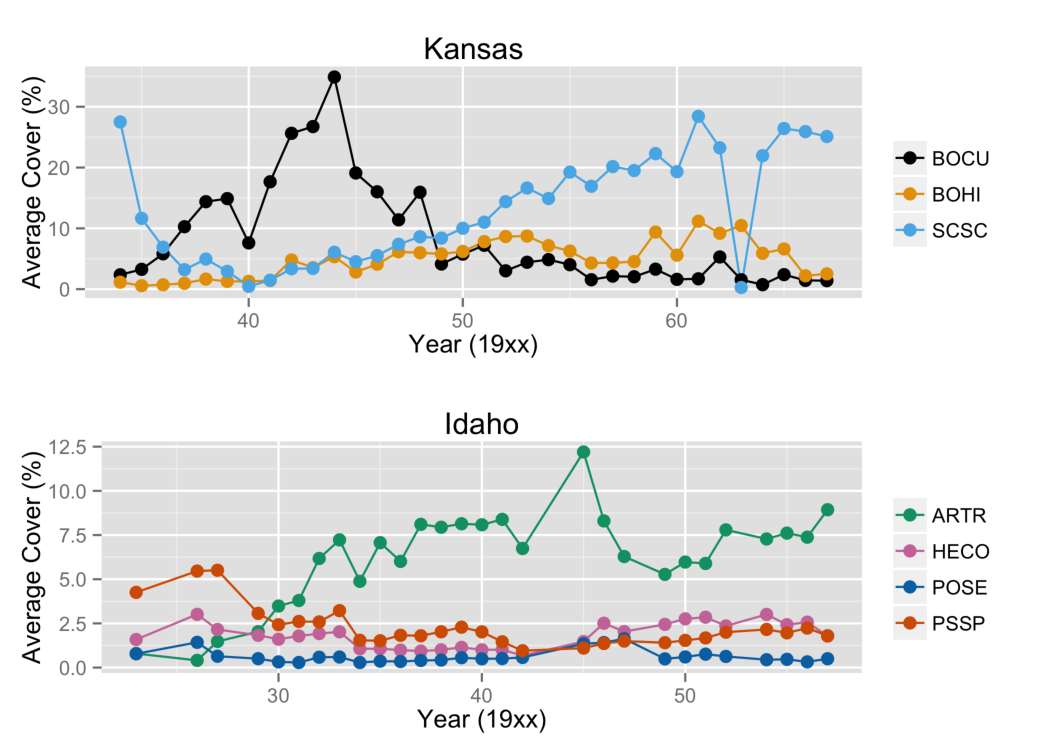
\includegraphics{components/figure/manuscript-figure_1.pdf}
\item
  Estimate community-wide synchrony using metric of Loreau and de
  Mazancourt (2008): \[
  \phi_{C} = \frac{\sigma_{C}^2}{(\sum\sigma_{i}^2)}
  \] We do this for species' percent cover, averaged over all the plots.
\end{enumerate}

\end{document}
